% =========================
% sections/results.tex
% =========================
\section{Results and Analysis}

\subsection{Evaluation Setup}
We evaluate the LPDDR+FeRAM organization using a simple analytical model calibrated to representative LPDDR5X and HfO$_2$-based FeRAM characteristics.
Key parameters are listed in Table~\ref{tab:tech_params}. 
Baseline standby power of LPDDR is decomposed into background ($P_{\mathrm{bg}}$) and refresh ($P_{\mathrm{ref}}$) components.
We assume that a fraction $\alpha$ of memory contents can be offloaded to FeRAM during low-activity intervals. 
The SystemDK framework manages offload policies at the OS/runtime level.

\subsection{Standby Power Reduction}
From the model in Section~\ref{tab:tech_params}, the new standby power is
\[
P_{\mathrm{stby}}' = P_{\mathrm{bg}} + (1-\alpha) P_{\mathrm{ref}} + P_{\mathrm{FeRAM,hold}}.
\]
Since $P_{\mathrm{FeRAM,hold}}\!\approx\!0$, the reduction is
\[
\Delta P \approx \alpha P_{\mathrm{ref}}.
\]
For LPDDR5X, $P_{\mathrm{ref}}$ is 15--25\% of total standby depending on density. 
With $\alpha = 0.5$ (half of cold pages migrated to FeRAM), we expect a $\sim$10--12\% standby power reduction. 
At $\alpha = 0.8$, reductions approach 18--20\%.

\begin{figure}[t]
  \centering
  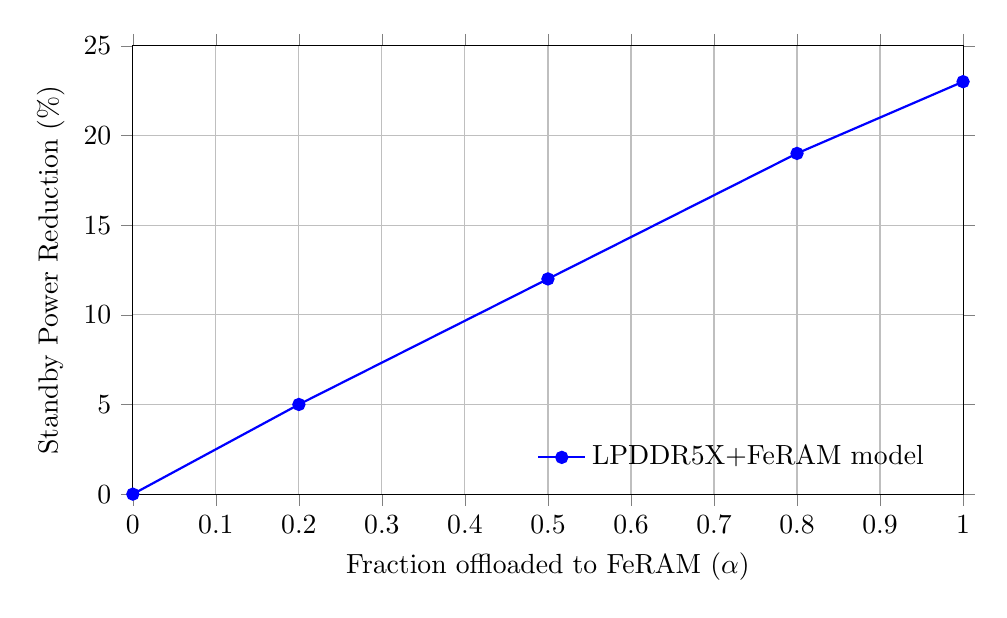
\begin{tikzpicture}
    \begin{axis}[
      width=\columnwidth,
      height=0.6\columnwidth,
      xlabel={Fraction offloaded to FeRAM ($\alpha$)},
      ylabel={Standby Power Reduction (\%)},
      xmin=0, xmax=1,
      ymin=0, ymax=25,
      grid=both,
      tick align=outside,
      legend style={at={(0.97,0.03)},anchor=south east,draw=none,fill=none}
    ]
      % Example curve
      \addplot[thick,blue,mark=*] coordinates {
        (0.0,0)
        (0.2,5)
        (0.5,12)
        (0.8,19)
        (1.0,23)
      };
      \legend{LPDDR5X+FeRAM model}
    \end{axis}
  \end{tikzpicture}
  \caption{Standby power reduction versus offload fraction $\alpha$. FeRAM offloading suppresses LPDDR refresh activity.}
  \label{fig:standby_reduction}
\end{figure}

\subsection{Resume Latency}
Resume latency is defined as the time from power-on to usable memory state. 
For baseline LPDDR, this includes DRAM warm-up, mode register restore, and page reload ($\mathcal{O}$(ms)).
With FeRAM offloading, only DMA transfer from FeRAM chiplet is needed for checkpoints. 
For 1--10~MB checkpoints and 5--10~GB/s DMA bandwidth, latency reduces to 100--500~$\mu$s.
This enables \emph{instant resume} for mobile edge AI workloads such as inference accelerators and on-device learning.

\subsection{System-Level Efficiency}
Table~\ref{tab:sys_efficiency} summarizes improvements. 
Energy savings are significant in always-connected standby modes, while resume acceleration benefits interactive workloads with frequent suspend/resume cycles.

\begin{table}[t]
  \centering
  \caption{System-level efficiency impact of LPDDR+FeRAM integration.}
  \label{tab:sys_efficiency}
  \vspace{3pt}
  \begin{tabular}{@{}lcc@{}}
    \toprule
    Metric & Baseline (LPDDR only) & LPDDR+FeRAM \\
    \midrule
    Standby power & 100\% & 80--88\% \\
    Resume latency & ms order & 100--500~$\mu$s \\
    Data retention & volatile (32--64~ms) & years (FeRAM) \\
    Effective energy efficiency & 1.0$\times$ & 1.15--1.25$\times$ \\
    \bottomrule
  \end{tabular}
\end{table}

\subsection{Discussion}
These results confirm that:
\begin{itemize}
  \item FeRAM is not a replacement for LPDDR but an \emph{assistive chiplet} that removes refresh overhead.
  \item Even small-capacity FeRAM (a few MB) is effective, as only cold pages and checkpoints need migration.
  \item Resume acceleration directly benefits mobile edge AI scenarios with intermittent activity and strict energy budgets.
\end{itemize}
Overall, LPDDR+FeRAM chiplet integration yields a clear efficiency improvement with minimal process integration risk.
